\subsubsection{Some simple calculations}

\begin{frame}{\subsubsecname}
    In \ab{} workflows, most calculations are done by \ab{} software.
    However, sometimes we do need to do some calculations by ourselves when preparing the input
    or analyzing the output, such as unit conversion, fitting, root-finding, and some more
    complicated computations.\\

    In \express{}, \texttt{EquationsOfStateOfSolids.jl} and \texttt{Crystallography.jl}
    are two good examples.
\end{frame}

\begingroup
\scriptsize % Change this page's font size, see https://tex.stackexchange.com/a/213839/61591
\begin{frame}[fragile]
    \frametitle{\subsubsecname}
    \framesubtitle{Fitting equations of state}

    A 3rd-order Birch--Murnaghan EOS needs 4 parameters: $V_0$, $B_0$, $B_0'$, and an optional
    $E_0$. From them, you can calculate $E(V)$, $B(V)$, and $P(V)$ of a solid material.

        {\tiny
            \begin{algorithmblock}
                \begin{juliaverbatim}
struct BirchMurnaghan3rd{T}
    v0::T
    b0::T
    b′0::T
    e0::T
    BirchMurnaghan3rd{T}(v0, b0, b′0, e0 = zero(v0 * b0)) where {T} = new(v0, b0, b′0, e0)
end
        \end{juliaverbatim}
            \end{algorithmblock}
        }

    How to distinguish different equations ($E(V)$, $B(V)$, $P(V)$)? Functions! Or,
    \href{https://docs.julialang.org/en/v1/manual/methods/#Function-like-objects-1}{function-like objects}.\\

    Evaluation:
    {\tiny
    \begin{algorithmblock}
        \begin{juliaverbatim}
eos = EnergyEquation(BirchMurnaghan3rd(224u"bohr^3", 9u"GPa", 4, -4400.3221128178u"eV"))
eos(29.6u"angstrom^3")  # -4399.983486835037u"eV"
        \end{juliaverbatim}
    \end{algorithmblock}
    }
    Notice how we do not need to convert between units! Thank god!\\

    Fitting equations of state:
    {\tiny
    \begin{algorithmblock}
        \begin{juliaverbatim}
nonlinfit(EnergyEquation(BirchMurnaghan3rd(40, 0.5, 4)), volumes, energies)
nonlinfit(EnergyEquation(Murnaghan1st(41, 0.5, 4)), volumes, energies)
nonlinfit(EnergyEquation(Vinet(41, 0.5, 4)), volumes, energies)
        \end{juliaverbatim}
    \end{algorithmblock}
    }
\end{frame}
\endgroup

\begin{frame}[fragile]
    \frametitle{\subsubsecname}
    \framesubtitle{Coordinate transformations in crystals}

    In crystallography, coordinate transformations are frequently used and liable to error.
    \begin{itemize}
        \item Crystal coordinates $\leftrightarrow$ Cartesian coordinates
        \item Primitive cell coordinates $\leftrightarrow$ standardized cell coordinates
    \end{itemize}

    \begin{columns}[t]
        \begin{column}[T, onlytextwidth]{0.2\textwidth}
            \begin{figure}
                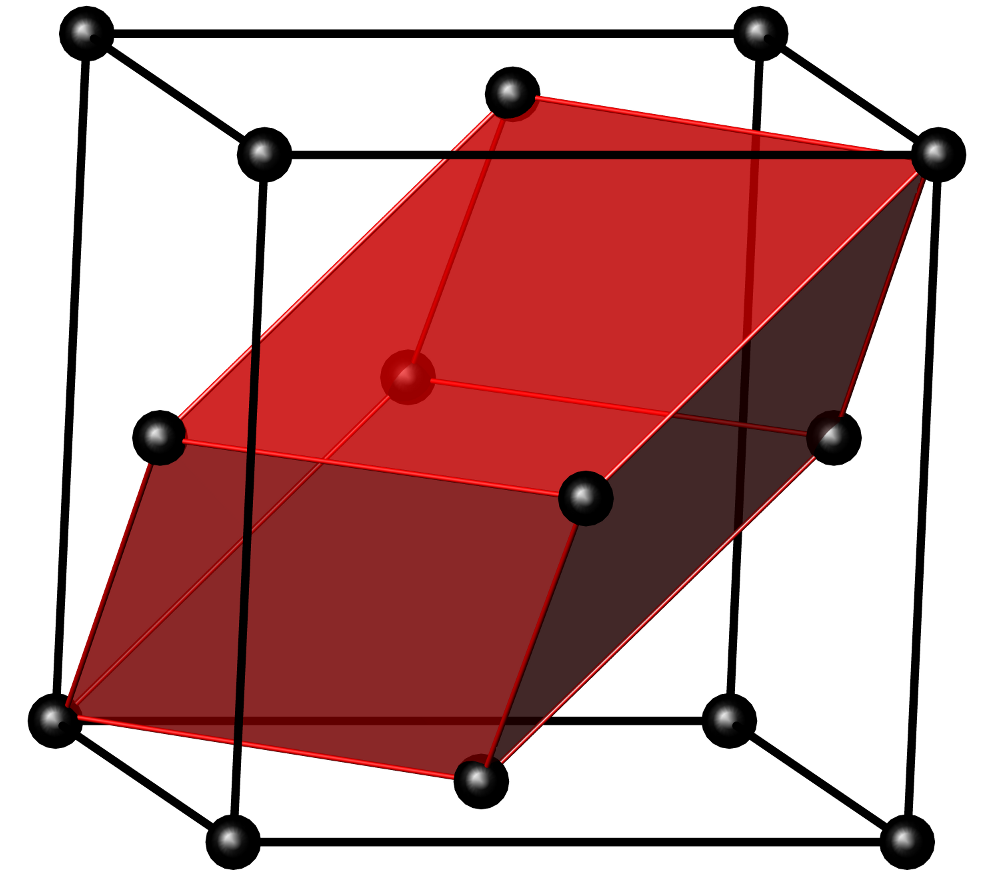
\includegraphics[width=\textwidth]{fcc}
                \captionsetup{font=tiny}
                \caption{Conventional (cube) \& primitive (red) cells of the FCC structure}
            \end{figure}
        \end{column}

        \begin{column}[T]{0.8\textwidth}
            {\scriptsize
                \begin{algorithmblock}
                    \begin{juliaverbatim}
using CoordinateTransformations: Transformation

struct CartesianFromFractional{T} <: Transformation
    tf::SMatrix{3,3,T,9}
end
struct PrimitiveFromStandardized{T} <: Transformation
    tf::SMatrix{3,3,T,9}
end
CartesianFromFractional(lattice::Lattice) = ...
(x::CartesianFromFractional)(v) = x.tf * collect(v)
(x::PrimitiveFromStandardized)(v) = inv(x.tf) * collect(v)
        \end{juliaverbatim}
                \end{algorithmblock}
            }
        \end{column}
    \end{columns}
\end{frame}
